\documentclass[fleqn, a4paper. 12pt]{jsarticle} 
\usepackage{cite}
\usepackage{amsmath,txfonts}
\usepackage{amssymb}
\usepackage{url}
\usepackage[margin=31mm]{geometry}
\usepackage[dvipdfmx]{graphicx}
\usepackage{listings,jvlisting}
\usepackage{fancyhdr}
\usepackage{lastpage}
\usepackage{hyperref}
\lstset{
  basicstyle={\ttfamily},
  identifierstyle={\small},
  commentstyle={\smallitshape},
  keywordstyle={\small\bfseries},
  ndkeywordstyle={\small},
  stringstyle={\small\ttfamily},
  frame={tb},
  breaklines=true,
  columns=[l]{fullflexible},
  numbers=left,
  xrightmargin=0zw,
  xleftmargin=3zw,
  numberstyle={\scriptsize},
  stepnumber=1,
  numbersep=1zw,
  lineskip=-0.5ex
}
\renewcommand{\lstlistingname}{プログラム}

% header
\pagestyle{fancy}
\fancyhf{}
\rhead{2024-05}
\lhead{谷 知拓 - Tomohiro Tani}
\cfoot{\thepage\ / \pageref{LastPage}}

\geometry{left=25mm,right=25mm,top=25mm,bottom=30mm}

\begin{document}

  \begin{titlepage}
    \begin{center}
      {\Huge 2024年度\\応用プログラミング実験}
      
      \vspace{4cm}
      {\Huge 第6-8回\\確率プログラミング\\
        実験レポート\\
      }
      \vspace{4cm}
      {\large 学修番号: 22140026\\谷 知拓 - Tomohiro Tani\footnote{東京都立大学 システムデザイン学部 情報科学科 \\ mail@taniii.com} \\}
      \vspace{0.5cm}
      {\large
        第1回レポート提出日 : 2024-05-22 \\
        第2回レポート提出日 : 2024-05-30 \\
        第2回レポート提出日 : 2024-06-06 \\
      }
    \end{center}
  \end{titlepage}

  \section*{はじめに}

    本レポートでは,『応用プログラミング実験』第6-8回の実施報告を行う.

  \subsection*{実験の概要}

    本実験では,確率プログラミングについて学ぶ.
    以下の課題に取り組み,その結果を報告する.

    \begin{enumerate}
      \item 課題1-1: 逆関数法による乱数生成
      \item 課題1-2: 逆関数法による乱数生成
      \item 課題1-3: ランダムウォーク
      \item 課題1-A: 線形合同法
    \end{enumerate}

  \subsection*{実験環境}

    実験環境は以下の通りである.

    \begin{itemize}
      \item OS\footnote{Operating System}: macOS Ventura 13.4.1
      \item CPU\footnote{Central Processing Unit}: Apple M2 arm64\footnotemark[4]
      \item メインメモリ・ビデオメモリ共通: 16GBユニファイドメモリ\footnotemark[4]
      \footnotetext[4]{https://www.apple.com/jp/macbook-air-13-and-15-m2/specs/}
      \item 実行環境 (rustc): rustc 1.78.0 (9b00956e5 2024-04-29)
      \item 実行環境 (cargo): cargo 1.78.0 (54d8815d0 2024-03-26)
    \end{itemize}

  \newpage
  \section*{課題1-1: 逆関数法による乱数生成}

    \texttt{kadai\_1\_1\_tomohiro\_tani.rs} を参照のこと.

    \quad

    なお,プログラムを実行して確認しやすくするために,上記プログラムと合わせて,依存関係の定義など実行に必要なファイルを含めたプロジェクトリポジトリ \texttt{rust} を添付している.

    実行方法は以下の通りである.

    まず,\texttt{rust} の実行環境は以下のコマンドでインストールすることができる.

    \begin{verbatim}
      curl --proto '=https' --tlsv1.2 -sSf https://sh.rustup.rs | sh
    \end{verbatim}

    各課題は, \texttt{works} モジュール内のサブモジュールに含まれているので, それぞれのサブモジュールの \texttt{main} 関数を呼び出すことで実行できる.

    各課題を実行するためには, \texttt{src} ディレクトリ直下の \texttt{main} 関数内で呼び出す関数を変更する.

    実行は,プロジェクトリポジトリ直下で,以下のコマンドで行うことでできる.

    \begin{verbatim}
      cargo run
    \end{verbatim}

  \newpage
  \section*{課題1-2: 逆関数法による乱数生成}

    \texttt{kadai\_1\_2\_tomohiro\_tani.rs} を参照のこと.

    \subsection*{概要}
    課題1-1で作成した関数\texttt{rnd\_exp}が,$\lambda$の指数分布に従う乱数を生成しているかを検証する.検証方法として,以下の2つの観点から理論値と比較する:
    \begin{enumerate}
        \item 乱数の平均値と分散
        \item 乱数の分布
    \end{enumerate}

    \subsection*{平均値と分散の検証}
    まず,$\lambda = 1.0, 1.5, 2.0$ の3つの異なるパラメータに対して,$n = 10,000$個の乱数を生成した.生成された乱数の平均値と分散を計算し,理論値と比較した.

    理論値は以下の通り:
    \begin{align*}
        \text{平均値} & : E[X] = \frac{1}{\lambda} \\
        \text{分散} & : V[X] = \frac{1}{\lambda^2}
    \end{align*}

    \quad

    シミュレーション結果と理論値の平均値及び分散を表 \ref{table:1}にまとめる.

    \begin{table}[h]
      \centering
      \caption{シミュレーション結果と理論値の比較}
      \begin{tabular}{|c|c|c|c|c|}
      \hline
      $\lambda$ & 平均値 (理論値) & 平均値 (シミュレーション) & 分散 (理論値) & 分散 (シミュレーション) \\
      \hline
      1.0 & 1.000 & 0.998 & 1.000 & 1.018 \\
      1.5 & 0.667 & 0.658 & 0.444 & 0.452 \\
      2.0 & 0.500 & 0.493 & 0.250 & 0.240 \\
      \hline
      \end{tabular}
      \label{table:1}
    \end{table}

    シミュレーション結果は理論値と高い精度で一致しており,\texttt{rnd\_exp}関数が正しく指数分布に従う乱数を生成していることが確認できた.

    \subsection*{分布の検証}
    次に,生成された乱数の分布をプロットし,理論的な確率密度関数と比較した.図 \ref{fig:1} 〜 図 \ref{fig:3} は,$\lambda = 1.0, 1.5, 2.0$ に対する確率密度関数と生成された乱数のヒストグラムを示している.

    \begin{figure}[!h]
      \centering
      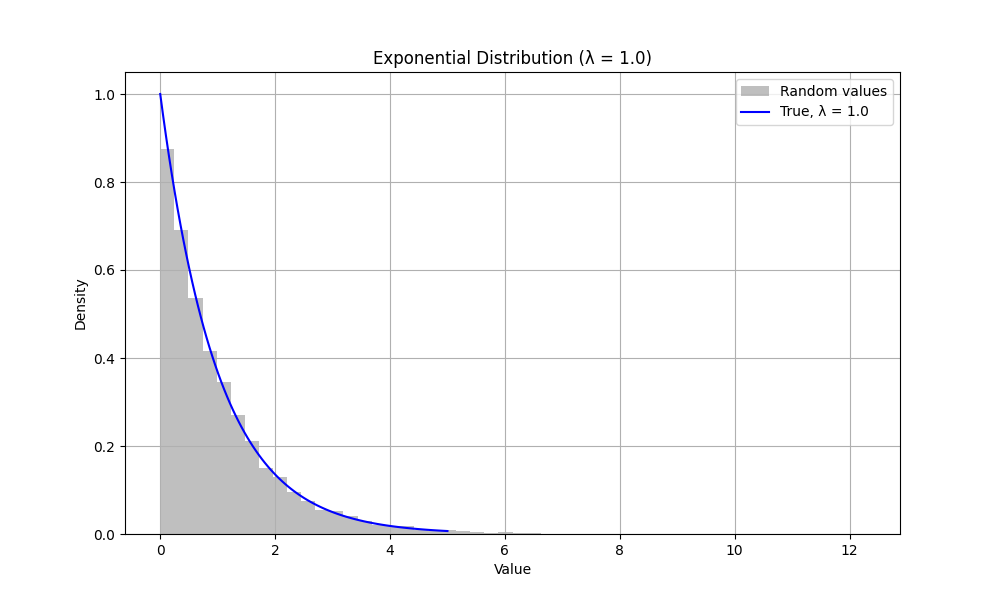
\includegraphics[width=0.6\textwidth]{lambda_1.0_plot.png}
      \caption{ $\lambda = 1.0$の指数分布}
      \label{fig:1}
    \end{figure}

    \begin{figure}[!h]
      \centering
      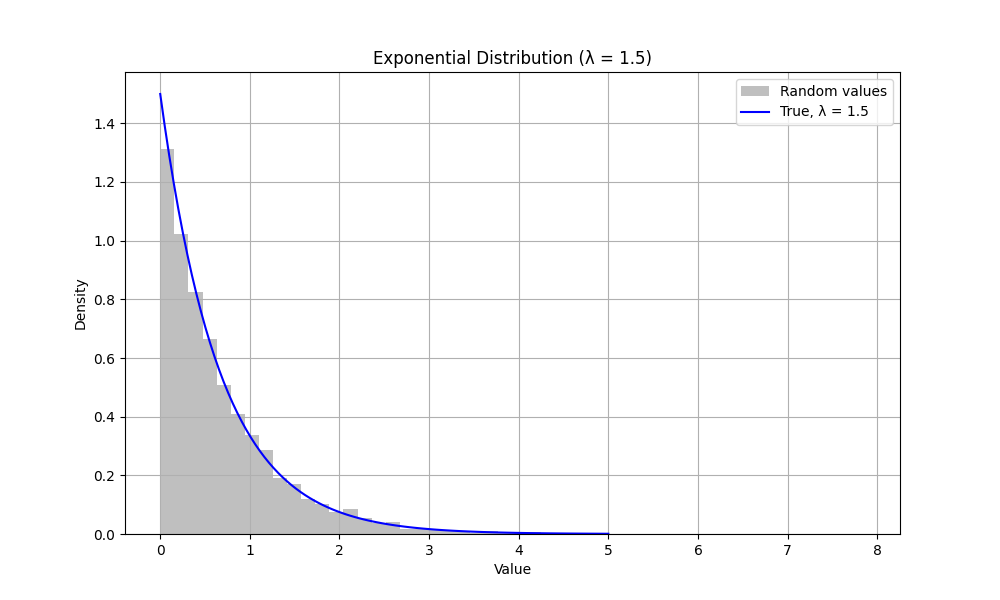
\includegraphics[width=0.6\textwidth]{lambda_1.5_plot.png}
      \caption{ $\lambda = 1.5$の指数分布}
      \label{fig:2}
    \end{figure}

    \begin{figure}[!h]
      \centering
      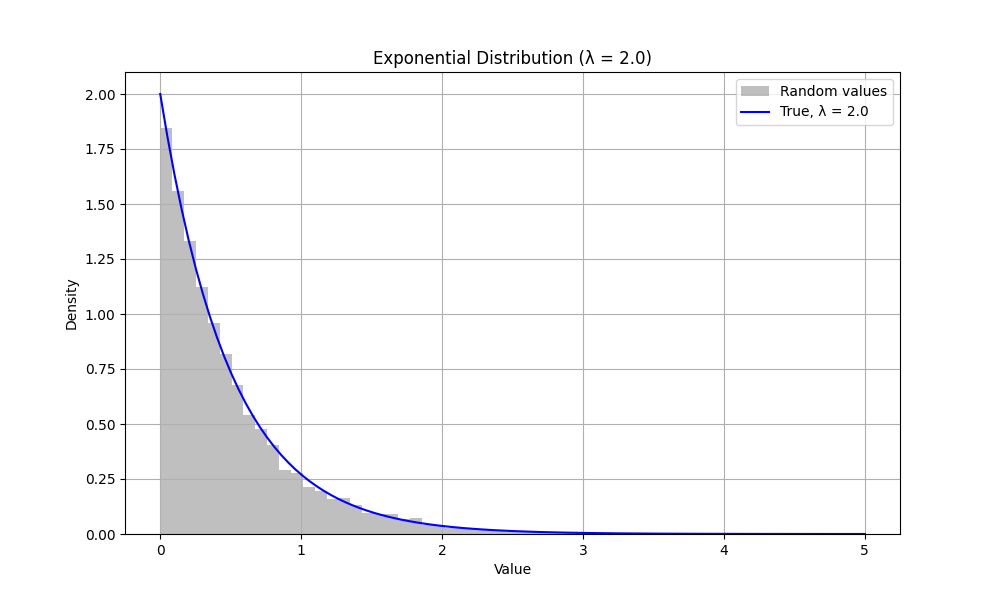
\includegraphics[width=0.6\textwidth]{lambda_2.0_plot.png}
      \caption{ $\lambda = 2.0$の指数分布}
      \label{fig:3}
    \end{figure}

    これらの図から,生成された乱数が理論的な指数分布に高い精度で一致していることが確認できる.

    \subsection*{考察}

      結果より,以下のように考察できる.

    \begin{itemize}
        \item 平均値と分散が理論値と高い精度で一致していることから,\texttt{rnd\_exp}関数が正しく動作していることが確認できた.
        \item 確率密度関数と乱数の分布が高い精度で一致していることから,生成された乱数が期待通りの分布に従っていることが確認できた.
        \item 逆関数法により,期待する確率分布に従う乱数を生成することができることが確認できた.
    \end{itemize}

  \newpage

  \section*{課題1-3: ランダムウォーク}

    \texttt{kadai\_1\_3\_tomohiro\_tani.rs} を参照のこと.

    \subsection*{概要}
    ランダムウォークのシミュレーションを行い,その結果を分析する.具体的には,$p = 0.5, d = 1$ の条件で1回のランダムウォーク(1000ステップ)の軌跡をプロットし,100回の独立なシミュレーションで得られる $t = 1000$ における点の位置 $S_{1000}$ の平均値と分散を計算する.
    
    \subsection*{結果}
    
    \subsubsection*{1回のランダムウォークの軌跡}
    図 \ref{fig:4} は,1回のランダムウォークで得られた点の位置 $S_t (t = 0, 1, ..., 1000)$ の軌跡を示している.
    
    \begin{figure}[h]
    \centering
    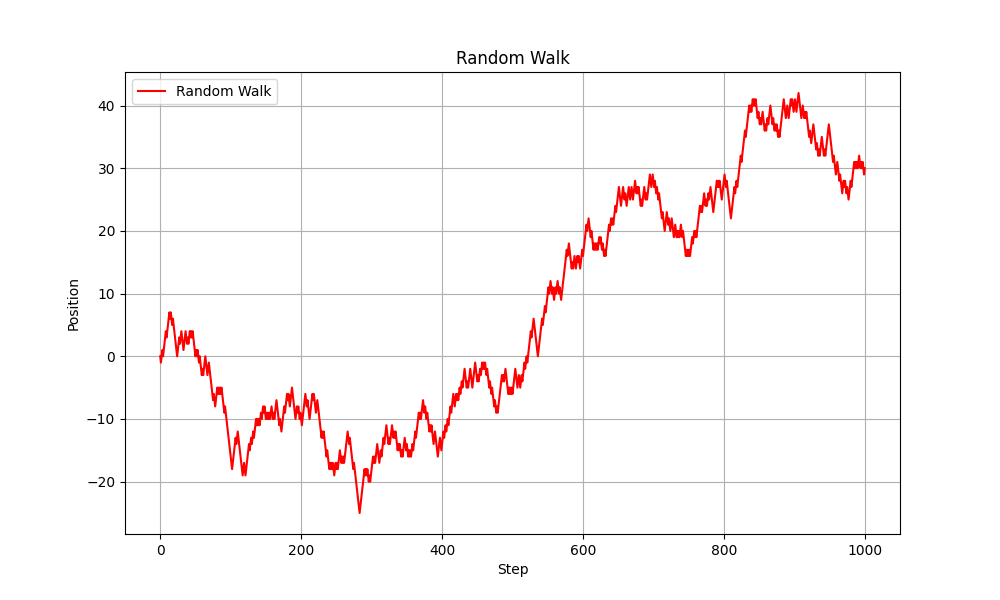
\includegraphics[width=0.8\textwidth]{random_walk_plot.png}
    \caption{ランダムウォークの軌跡}
    \label{fig:4}
    \end{figure}
    
    \subsubsection*{$S_{1000}$の平均値と分散}
    100回の独立なシミュレーションを行い,$t = 1000$における点の位置 $S_{1000}$ の平均値と分散を計算した.
    
    結果:
    \begin{itemize}
        \item 平均値: -1.080
        \item 分散: 1067.954
    \end{itemize}
    
    \subsection*{考察}
    \begin{itemize}
        \item \textbf{平均値について}: 理論的には,ランダムウォークの各ステップが独立であり,正負の方向に等確率で進むため,長期的な期待値は0となる.シミュレーション結果の平均値も0の近傍にあることから,矛盾しない.
        \item \textbf{分散について}: 理論的には,ランダムウォークの分散はステップ数に比例し,分散は $t \cdot d^2$ となる.今回のシミュレーションでは,$d = 1$であり,$t = 1000$のとき,分散は理論的には1000となる.シミュレーション結果の分散もこれに非常に近い値であるため,理論的な予測が正しいことが確認できた.
        ただし,$d$ をステップ毎の移動距離とする.
        \item \textbf{シミュレーションの信頼性について}: ランダムウォークのシミュレーション結果は理論的な期待値および分散と一致しており,このシミュレーション手法が信頼できるものであることがわかる.これにより,ランダムウォークを用いた複雑な現象のモデル化や解析が信頼性を持って行えることが示された.
    \end{itemize}
    
    これらの考察から,シミュレーションが理論的な予測と一致しており,乱数生成の品質が高いことが確認できた.ランダムウォークのモデルは,様々な分野における確率的現象の解析に有用であり,実験結果はその有効性を示しているといえる.
    
  \newpage

  \section*{課題2-1: ポアソン過程のイベントクラスの作成}

    \texttt{kadai\_2\_1\_tomohiro\_tani.rs} を参照のこと.

  \newpage

  \section*{課題2-2: ポアソン過程に従うイベント列を返す関数の作成}

    \texttt{kadai\_2\_2\_tomohiro\_tani.rs} を参照のこと.

  \newpage

  \section*{課題2-3: ポアソン過程のシミュレーション}

    \texttt{kadai\_2\_3\_tomohiro\_tani.rs} を参照のこと.

    \subsection*{概要}

      課題2-2で作成した関数を用いて,ポアソン過程のシミュレーションを行う.具体的には,$\lambda = 1.0, 1.5, 2.0$ のポアソン過程に従う $n = 100,000$ のイベント列を生成し,時間区間 $T = 1$ のイベント発生回数 $k$ の確率分布を考察する.

    \subsection*{結果}

      図 \ref{fig:5} 〜 図 \ref{fig:7} は,それぞれ $\lambda = 1.0, 1.5, 2.0$ のポアソン過程に従うイベント列を生成した結果である.

      ただし,折れ線は理論値,点はシミュレーション結果を示している.
      
      \begin{figure}[!h]
        \centering
        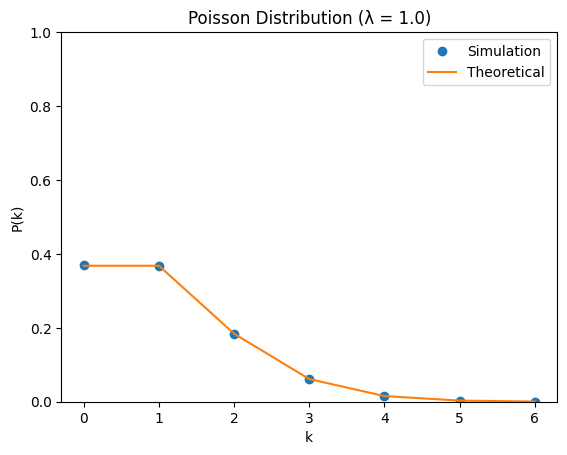
\includegraphics[width=0.6\textwidth]{5.png}
        \caption{時間区間 $T = 1$ のイベント発生回数 $k$ の確率分布 ($\lambda = 1.0$)}
        \label{fig:5}
      \end{figure}

      \begin{figure}[!h]
        \centering
        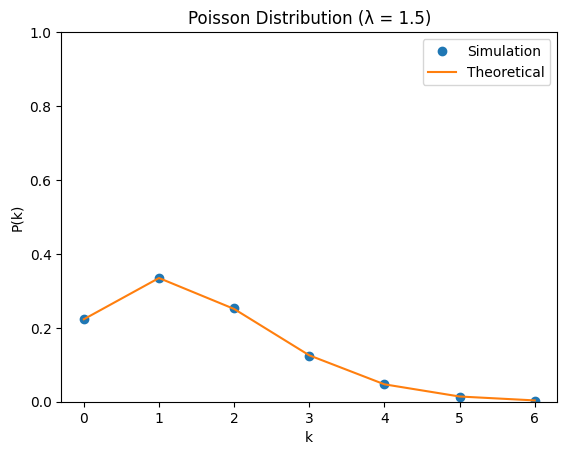
\includegraphics[width=0.6\textwidth]{6.png}
        \caption{時間区間 $T = 1$ のイベント発生回数 $k$ の確率分布 ($\lambda = 1.5$)}
        \label{fig:6}
      \end{figure}

      \begin{figure}[!h]
        \centering
        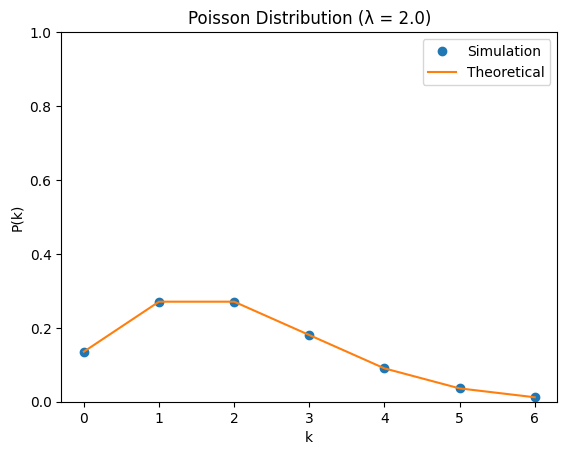
\includegraphics[width=0.6\textwidth]{7.png}
        \caption{時間区間 $T = 1$ のイベント発生回数 $k$ の確率分布 ($\lambda = 2.0$)}
        \label{fig:7}
      \end{figure}

    \subsection*{考察}

      結果より,以下のように考察できる.

      ただし,ポアソン過程の理論値は以下の式の通りである.

      \begin{equation}
        P(X = k) = \frac{e^{-\lambda} \cdot \lambda^k}{k!}
      \end{equation}

      \begin{itemize}
        \item \textbf{ポアソン過程の特性について}: ポアソン過程は,一定の時間区間内でのイベント発生回数がポアソン分布に従う確率過程である.シミュレーション結果は理論値と一致しており,ポアソン過程の特性が正しく再現されていることが確認できた.
        \item \textbf{パラメータ $\lambda$ について}: $\lambda$ が大きいほど,イベント発生回数の平均値が大きくなることが確認できた.また,$\lambda$ が大きいほど,イベント発生回数の分散も大きくなることが確認できた.これは,ポアソン過程の特性によるものであり,シミュレーション結果は理論的な予測と矛盾していないことがいえる.
      \end{itemize}

  \newpage

  \section*{課題3-1: M/M/S/S シミュレータの作成}

    \texttt{kadai\_3\_1\_tomohiro\_tani.rs} を参照のこと.

  \newpage

  \section*{課題3-2: M/M/1/1 シミュレーション}

    \texttt{kadai\_3\_2\_tomohiro\_tani.rs} を参照のこと.

    \subsection*{概要}

      課題 3-1 で作成した M/M/S/S シミュレータを用いて,M/M/1/1 シミュレーションを行う.
      
      具体的には,$\lambda = 2.0$ のときの,$\mu=1.5,1.6,1.7,1.8,1.9,2.0,2.1,2.2,2.3,2.4,2.5$ のロス率について求める.

    \subsection*{結果}

      図 \ref{fig:8} は,$\lambda = 2.0$ のときの,$\mu=1.5,1.6,1.7,1.8,1.9,2.0,2.1,2.2,2.3,2.4,2.5$ に対するロス率をグラフにしたものである.

      \begin{figure}[!h]
        \centering
        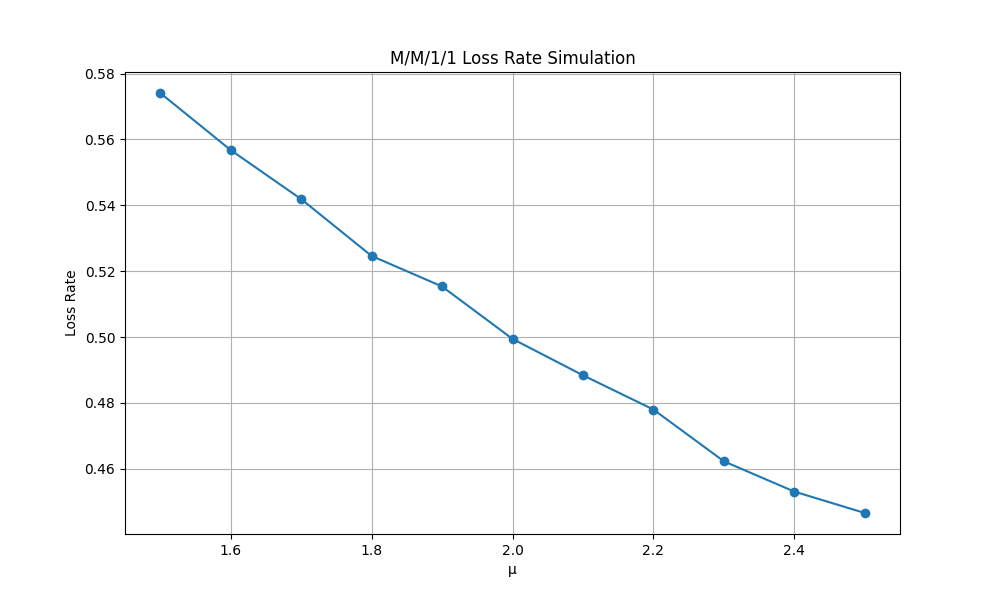
\includegraphics[width=1\textwidth]{plot_3_2.png}
        \caption{$\lambda = 2.0$ のときの,$\mu$ とロス率の関係}
        \label{fig:8}
      \end{figure}

    \subsection*{考察}

      このシミュレーションの理論値は以下の通りである.

      % 理論値
      \begin{equation}
        \text{理論値のロス率} = \frac{\lambda}{\lambda + \mu}
      \end{equation}

      \quad

      図 \ref{fig:t1} は,理論値のグラフである.

      \begin{figure}[!h]
        \centering
        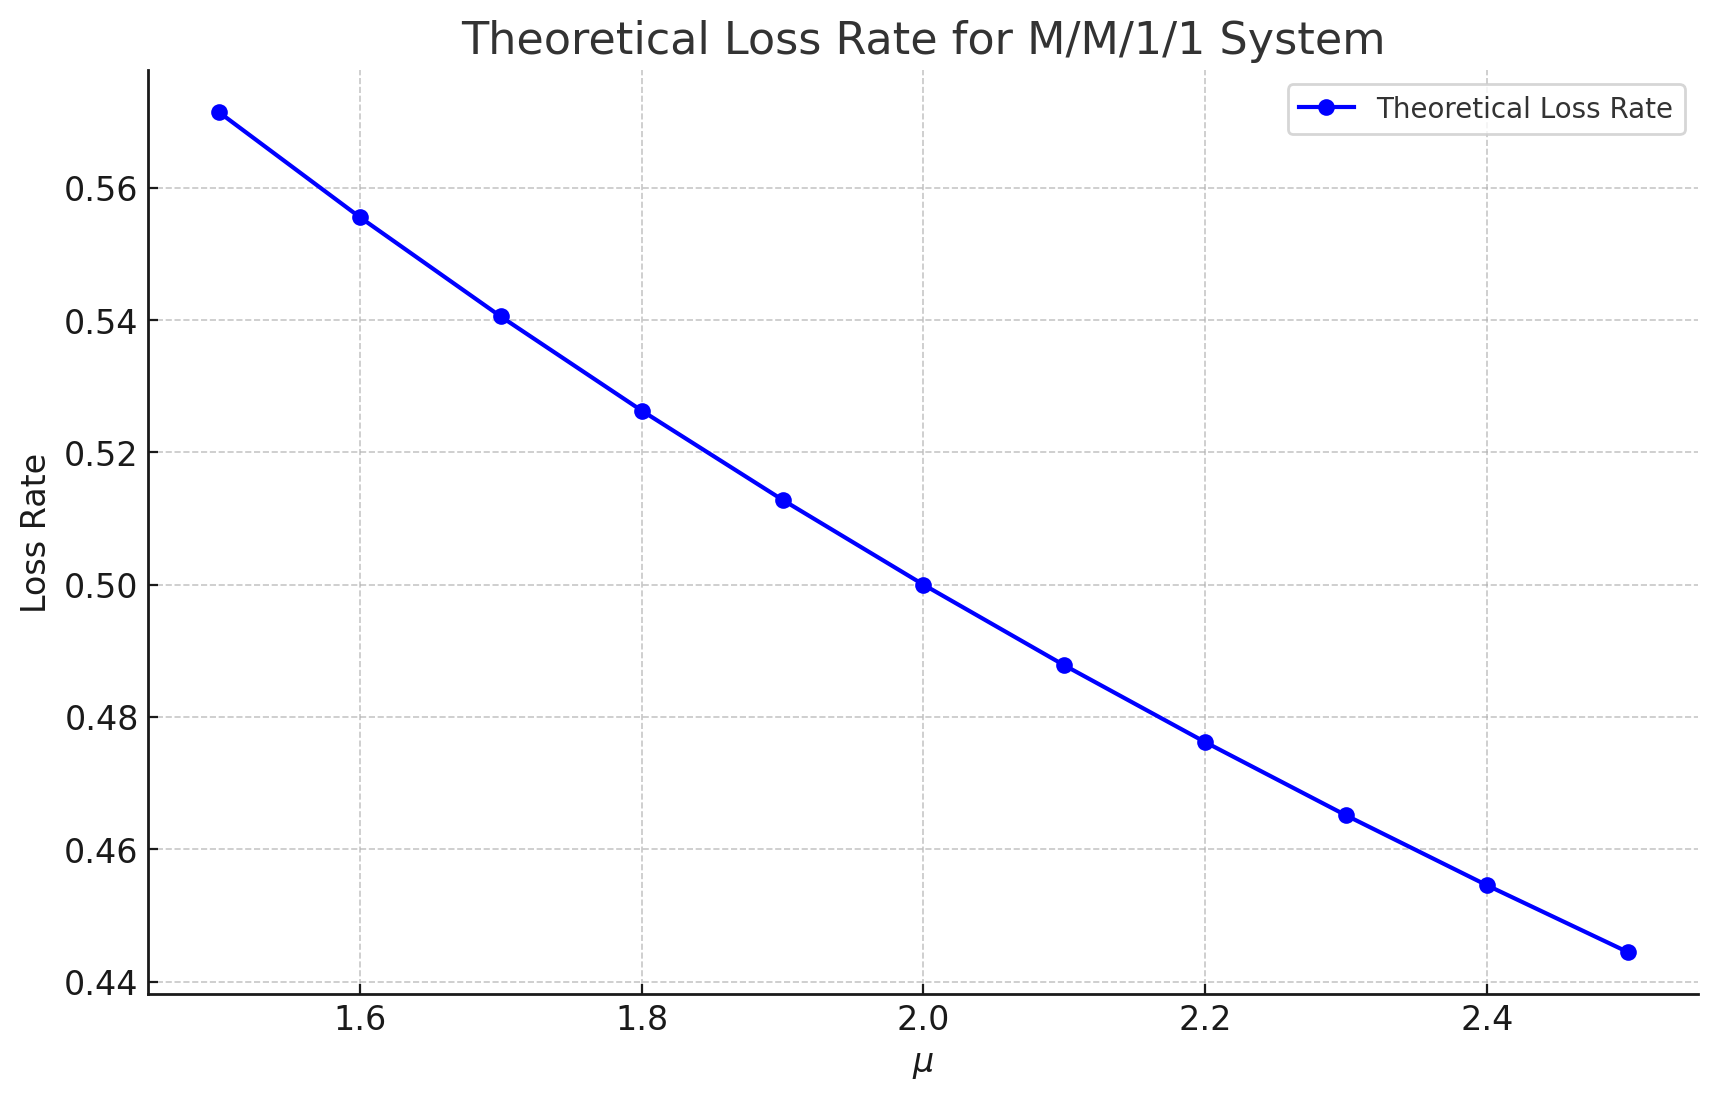
\includegraphics[width=0.9\textwidth]{t_3_2.png}
        \caption{$\lambda = 2.0$ のときの,$\mu$ とロス率の関係 (理論値)}
        \label{fig:t1}
      \end{figure}

      \quad

      図 \ref{fig:8} より,$\mu$ が大きいほど,ロス率が小さくなることが確認できる.これは,サービスの提供時間は $1/\mu$ に従う指数分布となるためであるといえる.

      また,図 \ref{fig:8} ,図 \ref{fig:t1} より,シミュレーション結果と理論値とは矛盾せず,正しいシミュレーションが行えたといえる.

  \newpage

  \section*{課題3-3: M/M/S/S シミュレーション}

      \texttt{kadai\_3\_3\_tomohiro\_tani.rs} を参照のこと.
  
      \subsection*{概要}
  
        課題 3-1 で作成した M/M/S/S シミュレータを用いて,M/M/S/S 待ち行列をモデル化したときのロス率のシミュレーションを行う.
        
      \subsection*{結果}
  
        図 \ref{fig:9} は,$S=1,2,3,4,5$ それぞれについて,$\lambda = 2.0$ とし,$\mu=0.5,0.6,0.7,0.8,0.9,1.0,1.1,1.2,1.3,1.4,1.5$ に対するロス率をグラフにしたものである.
  
        \begin{figure}[!h]
          \centering
          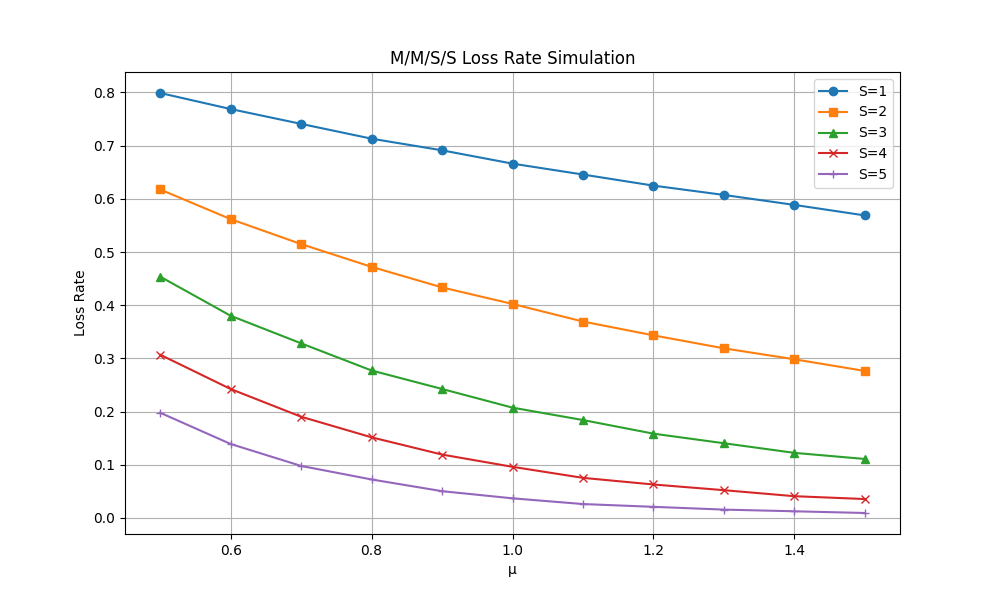
\includegraphics[width=1\textwidth]{plot_3_3.png}
          \caption{$S=1,2,3,4,5$ それぞれについて,$\lambda = 2.0$ とし,$\mu$ とロス率の関係}
          \label{fig:9}
        \end{figure}
  
      \subsection*{考察}
  
        図 \ref{fig:9} より,$S$ が大きいほど,ロス率が小さくなることが確認できる.これは,$S$ がサーバの数を表すためである.

        サーバの数が多いほど,リクエストを処理するキャパシティが大きくなるため,ロス率が小さくなることが理解できる.

    \newpage

    \section*{課題3-A: M/M/1/∞ シミュレーション}
  
      \texttt{kadai\_3\_4\_tomohiro\_tani.rs} を参照のこと.
  
      \subsection*{概要}
  
        課題 3-1 で作成した M/M/S/S シミュレータでは,サーバがすべて埋まっている場合にロスが発生する.
  
        ここでは,サーバがすべて埋まっている場合に,新たなリクエストが到着した場合に,任意のサーバに空きが生じるまで待機する M/M/1/∞ シミュレータを作成し,シミュレーションする.
  
        シミュレーションでは,$\lambda = 1.0, 1.5, 2.0, 2.5, 3.0$ のそれぞれのとき, $\mu = 0.5, 0.6, 0.7, 0.8, 0.9, 1.0, 1.1, 1.2, 1.3, 1.4, 1.5$ に対する待ち時間を求める.
        
      \subsection*{結果}
  
        図 \ref{fig:10} と表 \ref{table:2}, \ref{table:3} は,$\lambda = 1.0, 1.5, 2.0, 2.5, 3.0$ のそれぞれについて, $\mu = 0.5, 0.6, 0.7, 0.8, 0.9, 1.0, 1.1, 1.2, 1.3, 1.4, 1.5$ に対する待ち時間を試行したものである.
  
        \begin{figure}[!h]
          \centering
          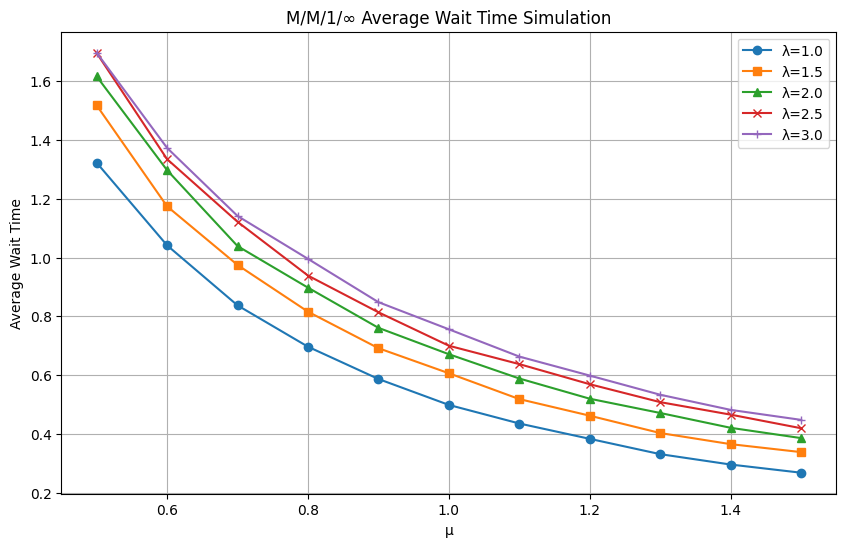
\includegraphics[width=1\textwidth]{plot_3_A.png}
          \caption{$\lambda = 1.0, 1.5, 2.0, 2.5, 3.0$ それぞれについて,$\mu$ と待ち時間の関係}
          \label{fig:10}
        \end{figure}

        \begin{table}[p]
        \centering
        \begin{tabular}{|c|c|c|}
        \hline
        $\lambda$ & $\mu$ & Average Wait Time \\
        \hline
        1 & 0.5 & 1.3228152698922535 \\
        1 & 0.6 & 1.041569830926313 \\
        1 & 0.7 & 0.8374044732034905 \\
        1 & 0.8 & 0.6967196489375518 \\
        1 & 0.9 & 0.5869698156477449 \\
        1 & 1 & 0.49875799140777366 \\
        1 & 1.1 & 0.43558179996194596 \\
        1 & 1.2 & 0.3833763555373002 \\
        1 & 1.3 & 0.33130003892426846 \\
        1 & 1.4 & 0.29597590419434566 \\
        1 & 1.5 & 0.2681681851815683 \\
        1.5 & 0.5 & 1.5179910691111629 \\
        1.5 & 0.6 & 1.1743131673277443 \\
        1.5 & 0.7 & 0.9748517752954529 \\
        1.5 & 0.8 & 0.8159103185325141 \\
        1.5 & 0.9 & 0.691728413085764 \\
        1.5 & 1 & 0.6064827751611467 \\
        1.5 & 1.1 & 0.5185512594446519 \\
        1.5 & 1.2 & 0.46209718876935896 \\
        1.5 & 1.3 & 0.40311204183920757 \\
        1.5 & 1.4 & 0.3653389920867382 \\
        1.5 & 1.5 & 0.3382454144182695 \\
        \hline
        \end{tabular}
        \caption{Average Wait Times for Different $\lambda$ and $\mu$ Values (Part 1)}
        \label{table:2}
        \end{table}

        \begin{table}[p]
        \centering
        \begin{tabular}{|c|c|c|}
        \hline
        $\lambda$ & $\mu$ & Average Wait Time \\
        \hline
        2 & 0.5 & 1.616443175247881 \\
        2 & 0.6 & 1.297284139505476 \\
        2 & 0.7 & 1.0390885645160224 \\
        2 & 0.8 & 0.8976514503134069 \\
        2 & 0.9 & 0.7609746883092575 \\
        2 & 1 & 0.6712300283393365 \\
        2 & 1.1 & 0.5886159523096386 \\
        2 & 1.2 & 0.5198381281538412 \\
        2 & 1.3 & 0.4713631072399001 \\
        2 & 1.4 & 0.4208963675680898 \\
        2 & 1.5 & 0.38592673299351204 \\
        2.5 & 0.5 & 1.6960399338643928 \\
        2.5 & 0.6 & 1.3348448122750503 \\
        2.5 & 0.7 & 1.1217175905202426 \\
        2.5 & 0.8 & 0.9387070482251122 \\
        2.5 & 0.9 & 0.8138929675559344 \\
        2.5 & 1 & 0.7001063316441805 \\
        2.5 & 1.1 & 0.6375614821933724 \\
        2.5 & 1.2 & 0.5691710428180768 \\
        2.5 & 1.3 & 0.5082233710422845 \\
        2.5 & 1.4 & 0.4656886944839204 \\
        2.5 & 1.5 & 0.41945248080787484 \\
        3 & 0.5 & 1.696860672213055 \\
        3 & 0.6 & 1.3730511708451394 \\
        3 & 0.7 & 1.1415333809844066 \\
        3 & 0.8 & 0.9955925998171699 \\
        3 & 0.9 & 0.8482943727529185 \\
        3 & 1 & 0.7559943425955813 \\
        3 & 1.1 & 0.6632060206479782 \\
        3 & 1.2 & 0.5985737201894004 \\
        3 & 1.3 & 0.5333848377164928 \\
        3 & 1.4 & 0.48189329603655956 \\
        3 & 1.5 & 0.4479137556725958 \\
        \hline
        \end{tabular}
        \caption{Average Wait Times for Different $\lambda$ and $\mu$ Values (Part 2)}
        \label{table:3}
        \end{table}

  
      \subsection*{考察}

        このシミュレーションの理論値は以下の通りである.

        % 理論値
        \begin{equation}
          \text{理論値の平均待ち時間} = \frac{\lambda}{\mu (\mu - \lambda)}
        \end{equation}
  
        図 \ref{fig:10} より,$\mu$ が大きいほど待ち時間が短く, $\lambda$ が大きいほど待ち時間が長くなることが確認できる.

        これは,$\rho=\frac{\lambda}{\mu}$ が混み具合を表すことからも理解できる.
  
        リクエストの到着率が大きく,サーバの処理時間 $1/\mu$ が長いほど,サーバがすべて埋まっている状態が続くため,待ち時間が大きくなることが理解できる.

  \newpage

  \section*{おわりに}

    第1回では,様々なシミュレーションをコンピュータを用いて行うには,期待する分布に従った乱数生成の手法が必要不可欠であることがわかった.
    
    また,乱数生成の品質がシミュレーション結果に大きな影響を与えるということを理解することができた.

    \quad

    第2回では,生成したイベントの発生回数の確率分布が,理論値とくるいなく一致しているのが印象的であった.

    世界のさまざまな事象をモデル化するのに,確率分布という概念が非常に重要であることがわかった.

    \quad

    第3回では,待ち行列のモンテカルロシミュレーションを行うことができ,特に Queue を用いた非同期処理システムをモデル化できたのがとても興味深かった.

    現在,開発業で,分散型メールシステムに関わる非同期処理システムの構築を行なっているため,今回の課題は非常に参考になった.

    具体的には,メールサーバからの取得プロトコルである,IMAP は 40 年近く前の 1986 年に誕生したため,現代の Webhook のようなステートレスにイベントを受け取る仕組みが十分でなく,最新のメールが来ていないかどうか,メールアカウントごとに確認しにいく必要があり,ここに非同期の待ち行列モデルが生じるため,設計に試行錯誤している.

  \newpage
  
  \section*{参考文献}

    \begin{itemize}
        \item Learn Rust - Rust Programming Language: \url{https://www.rust-lang.org/learn} (accessed: May 22, 2024)
    \end{itemize}

    \begin{itemize}
      \item Kleinrock, Leonard (1975). "Queueing Systems Volume 1: Theory"
    \end{itemize}

\end{document}